\documentclass[a4paper,12pt]{article}

\usepackage[utf8]{inputenc}
\usepackage[T1]{fontenc}
\usepackage[frenchb]{babel}
\usepackage{a4wide}
\usepackage{graphicx}
\usepackage{subfig}
\usepackage{tikz}
\usepackage{ifthen}
\usepackage{ifpdf}
\usepackage{comment}
\usepackage{listings} % pour code XML
\usepackage[babel=true]{csquotes}
\usepackage{float}

\usepackage{musixtex} % notation musicale
\usepackage{qtree} % pour faire des arbres rythmiques

\renewcommand{\familydefault}{\sfdefault}

\graphicspath{{images/}}

\newlength\figureheight
\newlength\figurewidth

\ifpdf
\usepackage[pdftex]{hyperref}
\else
\usepackage{hyperref}
\fi

\usepackage{color}
\hypersetup{
	colorlinks=true,
	linkcolor=black,
	citecolor=black,
	urlcolor=black
}

\renewcommand{\baselinestretch}{1.05}

%%%%%%%%% configuration du style fancy

\usepackage{fancyhdr}
\pagestyle{fancy}
\fancyfoot{}
\fancyhead[LE,RO]{\bfseries\thepage}
\fancyhead[RE]{\bfseries\nouppercase{\leftmark}}
\fancyhead[LO]{\bfseries\nouppercase{\rightmark}}
\setlength{\headheight}{15pt}

\let\headruleORIG\headrule
\renewcommand{\headrule}{\color{black} \headruleORIG}
\renewcommand{\headrulewidth}{1.0pt}
\usepackage{colortbl}
\arrayrulecolor{black}

\fancypagestyle{plain}{
  \fancyhead{}
  \fancyfoot[C]{\thepage}
  \renewcommand{\headrulewidth}{0pt}
}

%\makeatletter
%\def\cleardoublepage{\clearpage\if@twoside \ifodd\c@page\else
%  \hbox{}
%  \thispagestyle{empty}
%  \newpage
%  \if@twocolumn\hbox{}\newpage\fi\fi\fi}
%\makeatother

\parskip=5pt


\usepackage{amsthm}
\usepackage{array}
\usepackage{bm}

\lstset{ % encadrer et coloriser un document XML
  language=xml,frame=single, 
  breaklines=true, 
  basicstyle=\ttfamily,
  basicstyle=\scriptsize, 
  keywordstyle=\color{blue}, 
  commentstyle=\color{green}, 
  stringstyle=\color{red}, 
  identifierstyle=\color{blue}
}



\begin{document}

%%%%%%%%%%%%%%%%%%%%%%%%%%%%%%%%%%%%%%%%%%%%  page de garde  %%%%%%%%%%%%%%%%%%

\begin{titlepage}
\begin{center}

\begin{minipage}[c]{.46\linewidth}
  \centering
  
\includegraphics[width=0.6\textwidth]{logo_UPMC.png}\\[1cm]
\end{minipage}
\hfill
\begin{minipage}[c]{.46\linewidth}
  \centering
  
\includegraphics[width=0.5\textwidth]{logo_ircam.png}\\[1cm]
\end{minipage}

\vspace*{1cm}

{\large Université Pierre et Marie Curie}\\[1cm]

{\large Master Informatique, Spécialité STL}\\[1cm]

{\large Semestre 2, UE Projet STL}\\[1cm]

% titre
\rule{\linewidth}{0.5mm} \\[0.5cm]
{ \huge \bfseries Un analyseur syntaxique pour MusicXML \\[0.4cm] }
\rule{\linewidth}{0.5mm} \\[0.5cm]

\vspace*{1cm}

% Auteurs
\noindent
\begin{minipage}{0.5\textwidth}
  \begin{flushleft} \large
    \emph{Auteurs :}\\
      Sébastien DUCHENNE\\
      Alexandre GASPARD CILIA\\~\\
    \emph{Encadrant :} \\
    Pr.~Carlos AGON\\
  \end{flushleft}
\end{minipage}

\vspace*{2cm}


\vfill

\end{center}
\end{titlepage}


\newpage\null\thispagestyle{empty}\newpage


\tableofcontents

\newpage\null\thispagestyle{empty}\newpage

%%%%%%%%%%%%%%%%%%%%%%%%%%%%%%%%%%%%%%%%%%%%%%%  Remerciements  %%%%%%%%%%%%%%%%%%%%


\section{Remerciements}

Nous souhaitons remercier notre encadrant Carlos Agon qui nous a beaucoup aidé lors de ce projet. Ses cours de musique et une petite visite de l'IRCAM nous ont permis de découvrir ce domaine que nous connaissions peu. Ses idées et ses conseils nous ont aussi beaucoup apporté pour la réalisation du programme.

\par
Nous remercions également Karim Haddad pour ses explications de quelques éléments de la musique.


\newpage\null\thispagestyle{empty}\newpage

%%%%%%%%%%%%%%%%%%%%%%%%%%%%%%%%%%%%%%%%%%%%%%%  Liste des figures  %%%%%%%%%%%%%%%%%%%%


\listoffigures % liste des figures

\newpage\null\thispagestyle{empty}\newpage


%%%%%%%%%%%%%%%%%%%%%%%%%%%%%%%%%%%%%%%%%%%%%%%  Abbréviation  %%%%%%%%%%%%%%%%%%%%

%\begin{abbreviations}{ll} % liste des abbréviations

%\textbf{DOM} & \textbf{Document} \textbf{O}bject \textbf{M}odel\\
%\textbf{XML} & E\textbf{x}tensible \textbf{M}arkup \textbf{L}angage\\

%\end{abbreviations}


%%%%%%%%%%%%%%%%%%%%%%%%%%%%%%%%%%%%%%%%%%%%%%%  Contenu  %%%%%%%%%%%%%%%%%%%%


\pagestyle{fancy}

\section{Introduction}


L'IRCAM \cite{ircam}, Institut de Recherche et Coordination en Acoustique/Musique, est un centre de création et de recherche scientifique sur la musique. Il a été fondé en 1969 par Pierre Boulez à la demande du président Georges Pompidou. 

\par
En 1995, le CNRS et le ministère de la Culture et de la Communication s'associe et créée l'UMR 9912 STMS. Cette unité mixte de recherche, hébergée à l'IRCAM, s'intéressent aux sciences et aux technologies de la musique et du son. En 2010, elle est rejoint par l'UPMC.

\par
Cette UMR est composé de nombreuses équipes de recherche. L'une d'elles s'intitule "Représentation musicale", et réalise des outils de compositions musicales. Elle a notamment créée OpenMusic \cite{openmusic}, un environnement de composition musicale assisté par ordinateur.

\par
Les chercheurs de l'IRCAM souhaitent travailler sur des partitions musicales sous formes d'arbres rythmiques. Actuellement, ils utilisent OpenMusic. Cependant, ce logiciel --- (mettre inconvénients) ---. C'est pourquoi, ils souhaitent une nouvelle version. 

\par
Ce programme sera écrit en langage Java et sera similaire à OpenMusic. Il permettra donc d'éditer graphiquement des morceaux de musique. Son implémentation comportera différents modules, dont celui consistant à construire les arbres rythmiques à partir d'un fichier au format MusicXML. C'est ce module que notre tuteur de projet Carlos Agon, enseignant-chercheur à l'UPMC et membre de l'équipe de représentation musicale, nous a demandé de réaliser.

\par
Le module que nous avons développé est déposé sur un compte GitHub \cite{github_pstl}.

\section{Technologies utilisées}

\subsection{OpenMusic}

OpenMusic \cite{openmusic} est un langage de programmation visuel basé sur le langage Lisp qui permet d'écrire graphiquement des compositions musicales. Il a été conçu par les chercheurs de l'IRCAM Carlos Agon, Gérard Assayag et Jean Bresson. Les programmes sont constitués d'éléments reliés entre eux et représentant des structures de données ou des fonctions. La figure suivante montre l'interface du logiciel.


\begin{figure}[!h] %h : here
\centering
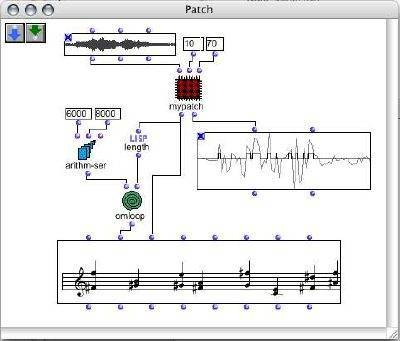
\includegraphics[width=0.8\textwidth]{openmusic.jpg}\\[1cm]
\caption{OpenMusic}
\label{OpenMusic}
\end{figure}

\par
Dans ce logiciel, les morceaux de musique sont constitués d'une suite d'arbres rythmiques. Comme décrit dans l'article \cite{agon}, \enquote{un arbre rythmique est défini comme un couple (D S) où D est une fraction (< 0) et S est une liste de n-éléments définissant n-proportions de D. Chaque élément de S peut-être soit un entier, soit un arbre rythmique.}

\par
Les images suivantes sont des exemples d'arbres rythmiques, en haut, et la partition correspondante, en bas.


\begin{minipage}[c]{.46\linewidth}
  \centering
  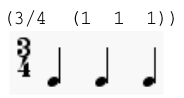
\includegraphics[width=0.5\textwidth]{rt1.png}\\[1cm]
\end{minipage}
\hfill
\begin{minipage}[c]{.46\linewidth}
  \centering
  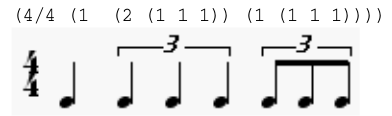
\includegraphics[width=0.9\textwidth]{rt2.png}\\[1cm]
\end{minipage}



\subsection{Le langage Java}

\par 
Java est un langage de programmation \textbf{orienté objet} fortement typé développé par \textbf{Sun Microsystems} à partir de \textbf{1995}. La société sera plus tard rachetée par \textbf{Oracle} en 2009 qui possède et maintient Java encore aujourd'hui.

\par 
Java se détache de la masse des autres langages de programmation notamment grâce à sa portabilité et sa facilité d'utilisation.

\begin{lstlisting}[caption=Hello world en java]
public class HelloWorld {
    public static void main(String[] args) {
        System.out.println("Hello world!");
    }
}
\end{lstlisting}

\par
Ci-dessus, un classique "Hello world" en Java. Nous pouvons y voir la définition de la classe \emph{HelloWorld} ainsi que la méthode principale du programme nommé \emph{main} et enfin un affichage sur la sortie standard.



\subsection{Le format MusicXML}

MusicXML \cite{musicxml} est un format de fichier permettant de représenter la notation musicale occidentale (notation classique, accords en notation anglo-saxonne, tablatures et percussions) et basé sur le langage XML. Il est propriétaire mais il peut librement utilisé avec une licence publique.

\par
Il y a plus de 20 ans, le format MIDI était très utilisé. Cependant, il n’est pas très adapté pour représenter toutes les caractéristiques de la musique, on perd donc en informations avec ce format. Pour pallier à cela, les formats SMDL et NIFF ont été créés. Cependant, le format SMDL était complexe et donc peu compréhensible. Il était donc très peu utilisé. Le format NIFF était un format peu pratique à utiliser et n’a donc pas été adopté par certains logiciels. Ces formats n’ont donc pas eu le succès souhaité.

\par
En 2004, la société Recordare LLC s’inspire des 2 formats universitaires MuseData et Humdrum pour créer la première version du format MusicXML. Ses avantages sont qu’il est facile à manipuler. Il permet le transfert de morceaux de musique d’une application à une autre. Il peut représenter beaucoup de caractéristiques de la musique. Cependant, il est verbeux, puisqu'il utilise le format XML, et ne donc permet pas de représenter la musique non occidentale.

\par
Il est de plus en plus utilisé puisque plus de 200 logiciels de musique l’ont adopté. Il est donc possible de travailler finement sur un morceau de musique en utilisant différents programmes.

\par
Comme le format XML est verbeux, le fichier prend de la place. La version 2.0, sortie en 2007, apporte donc la compression du fichier au format xml en un fichier au format mxl, et permet de diviser sa taille de façon importante. La version 3.0, sortie en 2011, permet le support des instruments virtuels.\\~\\

\par
On voit, dans le code correspondant à la partition suivante, que les informations sur la partition sont placées dans la balise "measure" et celle concernant la ronde sont contenues dans la balise "note".

\begin{figure}[!h] %h : here
\centering
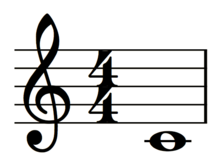
\includegraphics[width=0.2\textwidth]{musicxml_hello_world.png}\\[1cm]
%source : https://en.wikipedia.org/wiki/MusicXML
\caption{Hello World en MusicXML}
\label{Hello World en MusicXML}
\end{figure}


\begin{lstlisting}[caption=Document XML d'un Hello World en MusicXML, label=ruleml]
<?xml version="1.0" encoding="UTF-8" standalone="no"?>
<!DOCTYPE score-partwise PUBLIC
    "-//Recordare//DTD MusicXML 3.0 Partwise//EN"
    "http://www.musicxml.org/dtds/partwise.dtd">
<score-partwise version="3.0">
  <part-list>
    <score-part id="P1">
      <part-name>Music</part-name>
    </score-part>
  </part-list>
  <part id="P1">
    <measure number="1">
      <attributes>
        <divisions>1</divisions>
        <key>
          <fifths>0</fifths>
        </key>
        <time>
          <beats>4</beats>
          <beat-type>4</beat-type>
        </time>
        <clef>
          <sign>G</sign>
          <line>2</line>
        </clef>
      </attributes>
      <note>
        <pitch>
          <step>C</step>
          <octave>4</octave>
        </pitch>
        <duration>4</duration>
        <type>whole</type>
      </note>
    </measure>
  </part>
</score-partwise>
\end{lstlisting}



\subsection{Le langage XML}

Le langage XML \cite{xml_w3c, xml_ocr}, acronyme de e\textbf{X}tensible \textbf{M}arkup \textbf{L}angage, est langage de balisage générique spécifié par le W3C. Il permet de définir différents espaces de noms, c'est à dire des langages avec leur propre grammaire et vocabulaire. Il permet l'échange d'information entre des programmes très différents à condition d'utiliser la même grammaire.

\par
Il a l'avantage de pouvoir être compris par les êtres humains et les machines. Cependant, c'est un langage verbeux et qui peut donc prendre beaucoup de place s'il contient beaucoup d'information.

\par
Un document XML est constitué de balises pouvant contenir d'autres balises ou une valeur simple. Une balise peut aussi contenir des attributs donnant des informations supplémentaires sur le contenu.

\begin{lstlisting}[caption=Exemple d'un document XML]
<?xml version="1.0" encoding="UTF-8"?>
<racine>
    <balise attribut="valeur" >Contenu</balise>
    <baliseunique />
</racine>
\end{lstlisting}

\par
Ci-dessus un exemple de XML simpliste mais qui met en avant les bases du langage. La première ligne annonce le type de document et la version dans lequel le document va être rédigé. \emph{<racine>} est le nœud racine du document, celui qui en somme va contenir tout le document. On peut ici, facilement remarquer que le document peut être représenté sous la forme d'un arbre.

\par
XML permet à l'utilisateur de définir lui même la grammaire de son document grâce notamment aux \textbf{DTD} et au \textbf{Schéma XML}. Ces outils nous permettent de disposer de format d’échange de données tel que \textbf{MusicXML}.


\subsection{Le langage Relax NG}

\textbf{Relax NG} (\textbf{Re}gular \textbf{La}nguage for \textbf{X}ML \textbf{N}ext \textbf{G}eneration) née de la fusion de TreX de James Clark et de Relax de Murata Makoto. C'est un langage qui permet de définir la grammaire d'un document XML. Relax NG ne s'intéresse qu'à la structure du document et non à sa valeur.

\par
C'est ce que nous utiliserons afin de s'assurer de la validité du document à traiter.


\subsection{Affichage d'un graphe avec GraphStream}

Une fois le fichier XML parsé, nous disposons d'un \emph{DOM} sous forme d'un objet \emph{document}. Nous pouvons ensuite afficher l'arbre grâce à la librairie GraphStream \cite{graphstream}. Pour cela nous appelons un méthode qui affiche un nœud de l'arbre sur la racine du \emph{Document}. Cela nous permet donc d'afficher tout l'arbre.


\subsection{Les librairies}

Dans cette section, nous aborderons les librairies utilisées pour réaliser ce projet. Cela ira de la validation du XML en passant par le parsing de ce dernier, jusqu'à la récupération des information stockées dans le fichier MusicXML.


\subsubsection{Trang et Jing}

\textbf{Trang} \cite{trang} et \textbf{Jing} \cite{jing} sont deux librairies développées par \textbf{Thai Open Source}. Elles permettant de générer des grammaires Relax NG et de valider des documents XML à partir de cette même grammaire.

\par
Trang est une librairie qui permet de traduire un fichier de description grammaticale en fichier Relax NG. En effet XML n'est pas facilement lisible pour un esprit humain, c'est pour cela que Trang nous permet de créer notre grammaire dans un langage plus compréhensible. Une fois la grammaire écrite dans un fichier en \emph{.rnc}, nous pouvons générer notre fichier Relax NG en \emph{.rng}.

\par
Jing, quant à lui, est une librairie Java qui permet de valider un document XML à l'aide d'un fichier Relax NG.


\begin{lstlisting}[caption=Code java permettant de vérifier la validation d'un document XML]

final ValidationDriver vd = new ValidationDriver();
vd.loadSchema(rngFile);

if (!vd.validate(inputTextStream)) {
	throw new ParseException("Invalid xml :(");
} else {
    System.out.println("Valid xml :)");
}
\end{lstlisting}

\par
Le code ci-dessus est une utilisation simplifiée de Jing. Nous commençons tout d'abord par créer un objet \emph{ValidationDriver} de Jing dans lequel nous chargeons notre fichier Relax NG. Nous n'avons ensuite plus qu'à lancer la méthode \emph{validate(InputSource in) : boolean} qui nous indiquera si le document est valide.


\subsubsection{L'API SAX}

SAX \cite{sax_website, sax_oracle} est une API créée par David Megginson en 1998 et est l'acronyme de \textbf{S}imple \textbf{A}PI for \textbf{X}ML. Elle permet de manipuler des documents XML en utilisant des événements envoyées à chaque rencontre d'un élément.


\subsubsection{Le DOM}

Le DOM \cite{dom_w3c} , ou \textbf{D}ocument \textbf{O}bject \textbf{M}odel, est une interface de programmation normalisée par le W3C et est indépendant de tout plateforme et langage. Il voit les documents à balises comme des arbres dont le contenu et la structure peuvent être accédés et mis à jour dynamiquement.

\par
La figure suivante montre un exemple de DOM.

\begin{figure}[!h]
\centering
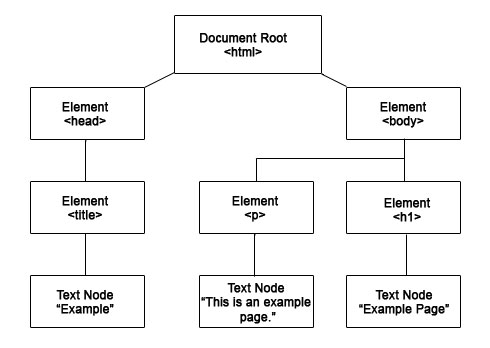
\includegraphics[width=0.8\textwidth]{ex_dom.jpg}\\[1cm]
%source : http://www.computerhope.com/jargon/d/dom.htm
\caption{Exemple d'un DOM}
\label{Exemple d'un DOM}
\end{figure}


\section{La notation musicale}

\subsection{La partition}


Une partition est un document contenant toutes les informations jugées nécessaires par l'auteur pour pouvoir interpréter une musique. Elle est composée de portées qui contiennent elles-même des mesures. Une mesure dispose d'une clé, d'une armure et d'une signature si elle est la première de sa portée et une ensemble de notes, accords ou silences.

\begin{figure}[!h]
\centering

\begin{music}
 
\instrumentnumber{1} % nombre de voix
\generalmeter{\meterfrac{4}{4}} % mesure 4/4
%\setname 1{chant} %nom de la portée
\generalsignature{3} % armure
 
\startextract
\metron{\qu}{60} % tempo
\NOTes\ha g\en %une blanche
%\NOTesp\qap g\en %une blanche pointée
\NOTes\hpause \en %une demi-pause

%\bar
%\Notes \islurd0c\qu{c d e}\tslur0f\qu f \enotes %liaison

\bar
%\Notes \ibu0d0\qb0{c c c}\tbu0\qb0d \enotes %beam
\Notes\qa g\en %une croche
\notes\Dqbu fg\en %beam double
\Notes\ibbbu0h0\qb0e\tbbbu0\qb0e\tbbu0\qb0e\tbu0\qb0e\en %beam 
\NOTes\zq c\zq e\zq g\qu j \en %accord
%\NOTes \zq{ceg}\qu j \en % autre manière de faire un accord

\endextract
 
\end{music}
 
\caption{Exemple d'une partition}
\end{figure}


\par
Une partition peut comporter plusieurs instruments ou voix. Une voix peut être formée de une (chant) ou deux portées (piano).

\begin{figure}[!h]
\centering 

\begin{music}
 
\instrumentnumber{2} % 2 instruments

\setstaffs 1{2} % instrument 1 (en bas) : 2 portées
 
\setclef{1}{60} % clef de fa (6) en 1, clef de sol (0) en 2
\generalmeter{\meterfrac{4}{4}} % mesure 4/4
\setname 1{piano} %
\setname 2{chant} %
\parindent 10mm % pour éviter la collision de piano avec l'accolade
 
\startextract
% {{bleu|1re mesure}}
\Notes 
\ha J | % chgt portée, même instr
\zhu{c e}\hu g & % chgt instr ; pas d'espace entre } et \hu
\ibu0d0\qb0{c c c}\tbu0\qb0d 
\enotes % assure l'alignement
%
\Notes 
\ha N | % chgt portée, même instr
\zhu{g i}\hu k & % chgt instr
\qa{e d} 
\enotes 
 
\bar % après toutes les notes de la mesure, pour toutes les voix
% {{bleu|2e mesure}}
\Notes
\qa J | 
\zqu{c e}\qu g &
\ibu0d0\qb0{c e} 
\enotes
%
\Notes
\qa N |
\zqu{g i}\qu k &
\qb0{d}\tbu0\qb0d
\enotes
%
\Notes
\ha J | 
\zhu{c e}\hu g &
\ha c 
\enotes
%
\endextract
 
\end{music}
 
\caption{Plusieurs portées et voix}
\end{figure}

\subsection{La durée}

La durée est le temps pendant laquelle la note est jouée. La durée n'est pas exprimée sous forme de valeur fixe mais comme une proportion relative à la mesure. En effet, la durée de la mesure dépend de sa signature et du tempo (expliqués plus tard). 


\subsection{La signature}

La signature symbolise le référentiel de la durée de la mesure. Elle peut être représentée sous forme d'une fraction. Le numérateur permet de définir la durée totale de la mesure et le dénominateur la durée d'un temps dans la mesure. 

\subsection{La note}

Une note est définie par sa hauteur et sa durée. La hauteur caractérise la fréquence du son d'une note. Cette fréquence est divisée en 8 intervalles appelé octave. Cette octave est divisée en 7 hauteurs : do, ré, mi, fa, sol, la et si. En ce qui concerne la durée de la note, elle est indiquée par la tête de la note et la présence ou non de symboles de croches. Si l'on ne prend pas en compte les croches, il existe 4 types de durées pour une note : carrée, ronde, blanche et noire. Une note carrée vaut 2 rondes, 4 blanches et 8 noires. Afin d'exprimer une durée plus courte que celle de la noire, on peut lui rajouter un ou plusieurs symboles de croches. La durée de la note s'en retrouve divisée par deux à chaque ajout.

\par
Dans notre programme, tout comme dans MusicXML, nous utilisons la notation anglo-saxonne. Elle diffère de la notation française par la façon dont est exprimée la hauteur et la durée de la note. Do, ré, mi, fa, sol, la et si sont remplacées respectivement par C, D, E, F, G, A et B. Concernant la durée, ce sont simplement des fractions. Par exemple, la blanche est un 1/2 (half) et la noire 1/4 (quarter).

\begin{figure}[!h]
  \centering
  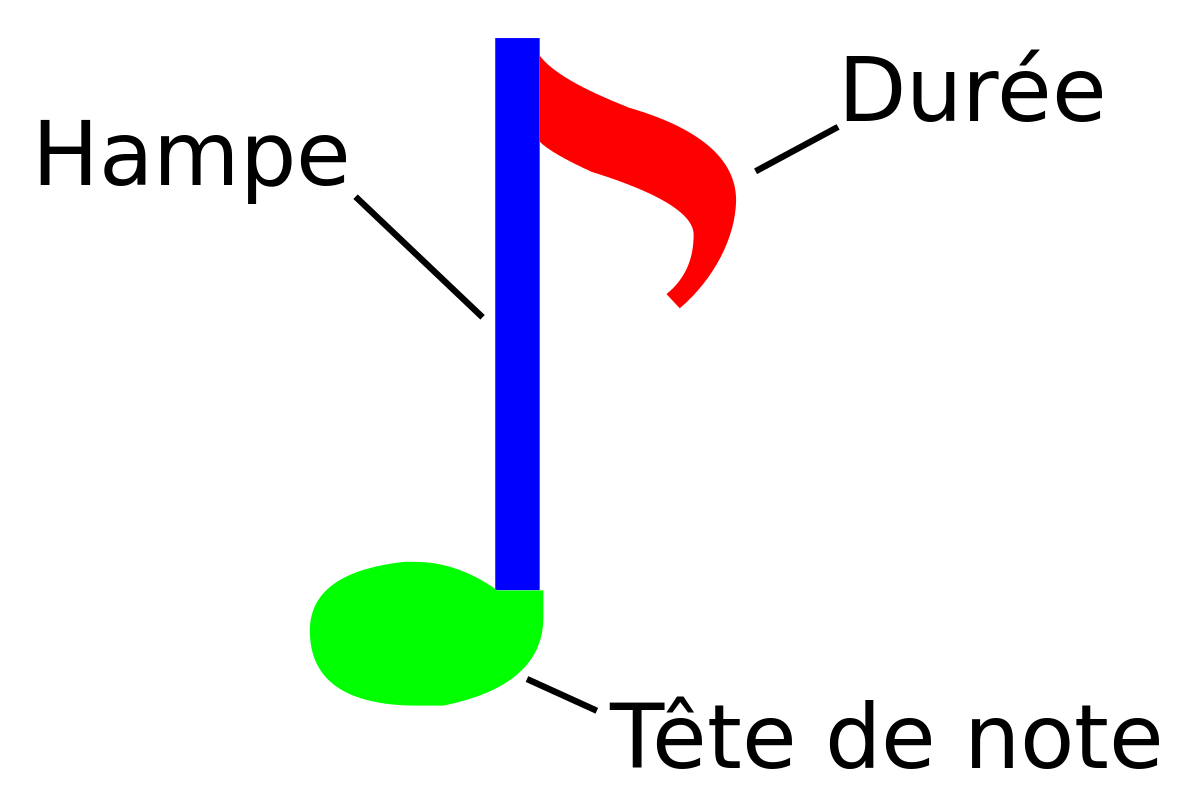
\includegraphics[width=0.3\textwidth]{note.png}\\[1cm]
  \caption{Symbole d'une note}
\end{figure}


\subsection{Le tempo}

Le tempo contient un type (une noire par exemple) et un nombre par minute. Ainsi, le tempo \emph{60 à la noire} signifie qu'il y a, dans une minute, 60 noires ou bien 30 blanches.


\subsection{Les symboles musicaux}

Nous désignons par symbole musical, chaque artefact influençant la manière de jouer une note ou un groupe de notes.

\par
Certains symboles ne s'appliquent que sur une figure de note. Ils sont dits unaires.

\begin{figure}[!h]
\centering

\begin{music}
 
\instrumentnumber{1}
 
\startextract
\NOTes \trrml j\ha j \en % tremolo double
\NOTes\en
\def\atnextbar{\znotes\loffset{0.7}{\centerbar{\Fermataup l\wh j}}\en}% point d'orgue

\bar
%accent
\Notes\ibu0f3\busfz0\qb0f\bupz0\qb0g\bust0\qb0h\buppz0\qb0i\busf0\qb0j\butext0\tqh0k\en
\Notes\Ibl0lg5\blsfz0\qb0l\blpz0\qb0k\blst0\qb0j\blppz0\qb0i\blsf0\qb0h\bltext0\tqb0g\en

\endextract
 
\end{music}
 
\caption{Symboles unaires}
\end{figure}

\par 
Les symboles influençant un groupe de notes sont appelés symboles binaires. Les 3 symboles suivant sont une liaison, un triolet et une appoggiature.
 
\begin{figure}[!h]
\centering 
 
\begin{music}
 
\instrumentnumber{1}
 
\startextract
\NOtes \islurd0g\qu g\tslur0g\qu g\en
\notesp \triolet n\isluru0l\Ibl0ln2\qb0{lm}\tslur0n\tqb0n\en % triolet
\notes \multnoteskip\smallvalue\smallnotesize\grcu j\en % petite note de l'appogiature
\NOTes \hu i\en
\endextract
 
\end{music}
 
\caption{Symboles binaires}
\end{figure}
 
 
Des symboles servent à répéter les notes d'une ou de plusieurs mesures.
 
\begin{figure}[!h]
\centering 

\begin{music}
 
\instrumentnumber{1}
 
\startextract
\NOTes\ha g\en
\leftrepeat
\NOTes\ha h\en
\leftrightrepeat
\NOTes\ha i\en
\rightrepeat
\NOTEs\wh j\en

\endextract
 
\end{music}
 
\caption{Symboles de répétitions}
\end{figure}



\subsection{L'arbre rythmique}

\par
Dans notre application, les durées des éléments constituant les mesures sont représentées sous forme d'arbres rythmiques. Comme décrit dans l'article \cite{agon}, \enquote{un arbre rythmique est défini comme un couple (D S) où D est une fraction (< 0) et S est une liste de n-éléments définissant n-proportions de D. Chaque élément de S peut-être soit un entier, soit un arbre rythmique.}


\par
Soit la partition suivante, constitué de deux noires et d'un soupir:

\begin{music}
 
\input musixps
\instrumentnumber{1}
\generalmeter{\meterfrac{3}{4}}
 
\startextract
\NOTes\qa g\en
\NOTes\qa g\en
\NOTes\soupir \en
\endextract
 
\end{music}

\begin{center}
(3/4 (1 1 -1) )
\end{center} 

\begin{figure}[!h]
\Tree[.3/4 [.1 ]
           [.1 ]
           [.-1 ]
     ]

\caption{Arbre rythmique 1}
\end{figure}



\par
Soit la deuxième partition suivante :

\begin{music}
 
\input musixps
\instrumentnumber{1}
\generalmeter{\meterfrac{2}{4}}
 
\startextract
\NOTes\qa g\en
\notesp\triolet n\Ibl0ln2\qb0{ll}\tqb0n \en % triolet
\endextract
 
\end{music}
 
\begin{center}
(2/4 (1 (1 (1 1 1) ) ) )
\end{center}  

\begin{figure}[!h]
\Tree[.2/4 [.1 ]
           [.1 
               [.1 ]
               [.1 ]
               [.1 ]
           ]
     ]

\caption{Arbre rythmique 2}
\end{figure}



%rt de silence et liaison



\section{Architecture du programme}
\par
Dans cette section nous aborderons l'architecture du programme. C'est-à-dire
la façon dont est organisé notre code et notamment les choix d'implementation
que nous avons effectués. Pour rappel, notre objectif est de générer un arbre rythique
et de récupérer la liste des accords et symboles musicaux pour réaliser l'affichage
de la partition musical.

\subsection{Architecture general}
\par
Le programme se divise en trois parties. La première étant le parser. Cette partie
permet au programme de disposer d'un \emph{DOM} à partir d'un fichier MusicXML.
La seconde partie est la représentation objet des données contenues dans le \emph{DOM}.
Et enfin la troisième partie est l'arbre rythmique qui pourra être généré à partir
de la représentation objet de la partition.

\subsection{Parsing du fichier MusicXML}
\par
La première étape est de parser le document afin d'extraire les informations qu'il
contient. C'est là qu'interviennent les éléments contenus dans le package
\emph{pstl.musicxml.parsing}. Nous avons décidé d'encapsuler le parser XML natif
de Java dans une class \emph{XMLParser}. Ce choix est motivé pour plusieurs raisons.
\par
Tout d'abord pour ne laisser apparent que les fonctions du parser de Java que
nous allons réellement utiliser afin de limiter le risque que nous ou un utilisateur
tiers fasse usage du parser d'une mauvaise façon. Nous avons aussi fait ce choix pour simplifier
l'utilisation de la class pour que la création du parser qu'elle encapsule se fasse de la même façon à chaque fois.
 Et enfin ce choix a été rendu nécessaire à cause de \emph{Relax NG}. En effet comme nous
ne faisons appel ni aux fichiers \emph{DTD} ni aux fichiers \emph{XML Schema}, il nous
faut effectuer un prétraitement pour éliminer les références aux \emph{DTD} du
fichier à parser. Vous pourriez vous demander pourquoi ne pas simplement
utiliser les \emph{DTD} pour valider le document ? La raison est simple,
la plupart des fichiers font référence aux \emph{DTD} en ligne fournis par
MusicXML. Or ces derniers n'autorisent que les navigateurs web à accéder à de tels
fichiers. Les possibilitées qui s'offraient à nous étaient les suivantes : se faire
passer pour un navigateur en modifiant quelques variables d'environement. Cela
aurait eu pour désavantage tout d'abord de ne pas être très rapide, l'accès à
aux \emph{DTD} par réseau n'est pas très rapide comparé à un accès local.
Nous jugions d'autre part la méthode peu honnête. En effet si l'organisation derrière MusicXML
ne permet pas cela pour des raisons que j'imagine financières (par cela j'entends le coût engendré par la maintenance des serveurs)
 il n'aurait pas été juste d'outrepasser leurs instructions. Et enfin le dernier choix non retenu était celui de faire appel
à des \emph{DTD} stockées localement. Cette méthode a été écartée bien que conseillée
dans la documentation du format MusicXML car elle impliquait des redirections d'URI
ce qui aurait fortement complexifié la création du parser.
\par %TODO Mettre reference vers le git de la grammaire rng de music xml
C'est donc pour toutes ces raisons que nous avons choisi d'utiliser \emph{Relax NG}.
De plus, les fichiers décrivants la grammaire de MusicXML sont disponibles en ligne
et l'auteur a fait preuve d'une certaine exhaustivité lors de la rédaction de ces derniers.
\par
Ce parser nous permet de disposer d'un \emph{DOM} (qui a pour nom de class \emph{Document} avec Java)
qui pourra être parcouru plus tard.

\subsection{Représentation objet de la partition}
\par
Nous aurions pu nous satisfaire du \emph{Document} retourné par le parser pour
générer notre arbre rythmique mais cela aurait posé plusieurs problèmes. Tout d'abord
la manipulation du \emph{DOM} n'est pas aisée. Cette structure de données basé sur
des noeuds qui contiennent des fils, attributs et leur contenu textuel, doit
être exploré d'une façon assez lourde à cause en partie du fait qu'un noeud n'est
pas nativement un objet iterable comme les \emph{Collections} de Java par exemple.
D'autre part, toutes les données contenues dans ces noeuds sont considérées comme des chaines
de caractère qui nécessitent un parsing et donc une manipulation assez verbeuse.
De ce fait, il est plus simple pour nous de parcourir ce \emph{Document} une seule fois et d'extraire les données qu'il
contient dans une structure de données plus aisément manipulable dans java. Cela
permet par exemple d'éviter des erreurs lors du développement des autres fonctionnalités de
l'application qui se basent sur ces informations.

%Mettre des figures pour expliciter les partitions ? Un diagramme de class par exemple ?
%TODO établir un vrai package pour les partitions.
\par
La structure de données que nous avons élaborée se compose de la façon suivante :
l'élément qui va contenir toutes les informations est la class \emph{Score}. Une
\emph{Score} contient une liste de \emph{Parts} qui l'on peut qualifier de
\emph{Voix} en français. Chaque \emph{Part} contient un nom, un identifiant ainsi qu'une liste
de \emph{Measures} (mesure) qui contient elle-même un numéro, une \emph{Signature} et une
liste de \emph{Chord} (accord). Un accord est composé d'une liste d'éléments musicaux
appelés \emph{MusicalItems} dans le programme. Chaque élément peut être soit une note
un silence ou une liaison. Un élément musical possède aussi une liste de symboles
musicaux. Un symbole musical représente une notation qui peut être une nuance comme
un point ou encore un répétition par exemple.
\par
On pourrait penser ce modèle de données lourd, mais cela est largement compensé entre autres
par l'aisance d'utilisation qu'il procure ainsi qui la possibilité notamment de déduire les
"coordonnées" des éléments qui le composent. En effet rien de plus facile que de dire
qu'une note se trouve dans le \emph{Chord} 4 de la \emph{Measure} 2 de la \emph{Part}
2 de telle \emph{Score}. Ainsi nous pouvons par exemple utiliser ces coordonnées pour
placer certains symboles à des endroits précis.

\section{Conclusion}

conclusion


%%%%%%%%%%%%%%%%%%%%%%%%%%%%%%%%%%%%%%%%%%%%%%%  Annexes  %%%%%%%%%%%%%%%%%%%%

%\appendix %

%\include{annexes}


%%%%%%%%%%%%%%%%%%%%%%%%%%%%%%%%%%%%%%%%%%%%%%%  Bibliographie  %%%%%%%%%%%%%%%%%%%%

\newpage\null\thispagestyle{empty}\newpage

\bibliographystyle{IEEEtran}
\bibliography{IEEEabrv,biblio}
\nocite{*}

\end{document}

